%!TEX root = ../report.tex

\begin{document}
    \justifying
    \chapter{Benchmarking}
    \label{Benchmarking}
    This chapter describes the detection datasets that are used to benchmark the current \acrlong{ood} (\acrshort{ood}) methods given an \acrlong{id} (\acrshort{id}) datasets, Metrics used to define the benchmark limits and the expected behavior from the \acrshort{ood} detector. 
    
    As mentioned in Section \ref{OOD_Detection} and shown in Figure \ref{fig:OOD_classes}, the \acrshort{ood} dataset should include images with considerable semantic shift either in the background of the image or in the objects present in the image. To establish a benchmark, we set the following requirements from our \acrshort{ood} detector which are adapted from the work done by \citet{Cao2020}.
    
    The \acrshort{ood} detector should be able to:
    \label{ood_cases}
    \begin{enumerate}
        \item Reject the image samples from a different domain. For example, images collected in a different country with very different road conditions from the image data used for training the object detection model.
        \item Reject low-quality images. For example, images with low contrast, improper lighting, motion blur, etc.
        \item Reject objects in the image which are unseen during the training. 
    \end{enumerate}

    \section{Datasets}
    Proposed frameworks to detect OOD samples used one dataset as ID and another dataset which is semantically very different from OOD. Adapting such a setting is not possible in the case of object detection, as the datasets available tend to be similar to others: the majority of the agents in the dataset tend to be similar. This section outlines the datasets utilized in this work, including the exploratory data analysis and the choices made to choose the training dataset.
    
    \subsection{Berkley Deep Drive (BDD100K) Dataset}
    \label{BDD100K_about}
    Berkley Deep Drive dataset which consists of 100,000 images, Hence this dataset is coined as BDD100K by \citet{bdd100k}. The collected images are annotated with object bounding boxes, road and object segmentation, lane-level markings, instance segmentation labels. The dataset is particularly wholesome as it covers various weather conditions (rainy, snowy, clear, overcast, partly cloudy, and foggy) as well as the various times in a day (daytime, night, dawn/dusk). This variance in the environment and illumination condition has made BDD100K a good and natural representation of a driving domain.
    
    The dataset consists of 1.8 million bounding boxes with objects belonging to 13 different classes ('pedestrian', 'rider', 'car', 'truck', 'bus', 'train', 'motorcycle', 'bicycle', 'traffic light', 'traffic sign', 'other vehicle','other person', 'trailer'). The distribution of Object-instances, average area of each Class-instance, Weather, and Time of Day are shown in Figure \ref{fig:OC_EDA}, Figure \ref{fig:OA_EDA}, Figure \ref{fig:Weather_EDA}, and Figure \ref{fig:TOD-EDA} respectively. Hence, we chose to use BDD100K dataset as In-Distribution dataset. 
    
    \begin{figure}[H]
        \includegraphics[width=.475\textwidth]{images/dataset_images/bdd01.jpg}
        % \includegraphics[width=.475\textwidth]{images/dataset_images/bdd02.jpg}
        % \\[\smallskipamount]
        % \includegraphics[width=.475\textwidth]{images/dataset_images/bdd04.jpg}\hfill
        \includegraphics[width=.475\textwidth]{images/dataset_images/bdd05.jpg}
        \caption[Sample images from \acrshort{bdd} dataset]{Example images from the \acrshort{bdd} datasets introduced by \citet{bdd100k}}
        \label{fig:bdd100k_samples}
    \end{figure}
    
    \begin{figure}[H]
         \centering
         \begin{subfigure}[b]{0.495\textwidth}
             \centering
             \includegraphics[width=\textwidth]{images/EDA/BDD100K_Weather_EDA.pdf}
             \caption[Weather samples count in \acrshort{bdd} dataset]{Weather count distribution}
             \label{fig:Weather_EDA}
         \end{subfigure}
         \hfill
         \begin{subfigure}[b]{0.495\textwidth}
             \centering
             \includegraphics[width=\textwidth]{images/EDA/BDD100K_timeofday_EDA.pdf}
             \caption[Time of Day samples count in \acrshort{bnn} dataset]{Time of day distribution }
             \label{fig:TOD-EDA}
         \end{subfigure}
            \caption{Weather and Illumination variations in BDD100K dataset}
    \end{figure}
    
    \begin{figure}[ht]
        \centering
        \includegraphics[scale=0.35]{images/EDA/BDD100K_objectcount_EDA.pdf}
        \caption[Object instances count in \acrshort{bdd} dataset]{Number of object instances for all the 13 classes present in BDD100K dataset with x-axis representing the count of object instances and y-axis representing the name of the object instance.}
        \label{fig:OC_EDA}
    \end{figure}
    
    \begin{figure}[ht]
        \centering
        \includegraphics[scale=0.35]{images/EDA/BDD100K_Average_Area_EDA.pdf}
        \caption[Average bounding box area vs Class name]{Plot representing average bounding box area per class}
        \label{fig:OA_EDA}
    \end{figure}
    
    
    \subsection{Indian Driving Dataset}
        Indian Driving Dataset is collected from very less structured environments around cities like Hyderabad, Bangalore in India. The road scenes differ highly from the environment with less structured traffic participants and a large variance in object types appears in the dataset. Figure \ref{fig:idd_samples} shows few random samples from the \acrshort{idd} dataset. 
        
    % \begin{figure}
    %     \centering
    %     \includegraphics[scale=0.2]{images/Indian_Driving_Dataset_Class_frequency.pdf}
    %     \caption{Plot representing average bounding box area per class}
    %     \label{fig:OA_EDA}
    % \end{figure}
        
    \begin{figure}[H]
        \includegraphics[width=0.5\textwidth]{images/dataset_images/IDD01.jpg}\hfill
        \includegraphics[width=0.5\textwidth]{images/dataset_images/IDD04.jpg}
        \caption[Sample images from \acrshort{idd} dataset]{Example images from the \acrshort{idd} dataset introduced by \citet{Varma2019IDDAD}}
        \label{fig:idd_samples}
    \end{figure}
    
    \begin{figure}[H]
        \centering
        \includegraphics[scale=0.35]{images/Indian_Driving_Dataset_Class_frequency.pdf}
        \caption[Instance count of \acrshort{idd} dataset]{Number of object instances for all the classes present in \acrshort{idd} dataset with x-axis representing the count of object instances and y-axis representing the name of the object instance.}
        \label{fig:IDD_EDA}
    \end{figure} 
    
    The reasons for using \acrshort{idd} as \acrshort{ood} dataset are
    \begin{enumerate}
        \item The Figures \ref{fig:bdd100k_samples} and \ref{fig:idd_samples} show that the road and driving conditions in which \acrshort{idd} dataset is recorded is very different from \acrshort{bdd} dataset. Thus making \acrshort{idd} dataset an out-of-domain dataset.
        \item The intra-class variance among the classes in \acrshort{idd} dataset is very high. For example the OOD detector should assign a high novelty score to a car in Figure \ref{magic} compared to cars in Figure \ref{Indica} - \ref{traveller}.  
        
        \begin{figure}[H]
            \centering
            \begin{subfigure}[b]{0.2\textwidth}
               \includegraphics[width=\textwidth]{images/dataset_images/idd_samples/Tata_Indica.jpg}
               \caption{i}
               \label{Indica}
            \end{subfigure}
            % \hfill
            \begin{subfigure}[b]{0.2\textwidth}
               \includegraphics[width=\textwidth]{images/dataset_images/idd_samples/Tata_sumo.jpg}\hfill
               \caption{ii}
               \label{sumo}
            \end{subfigure}
            % \hfill 
            \begin{subfigure}[b]{0.2\textwidth}
               \includegraphics[width=\textwidth]{images/dataset_images/idd_samples/Tempo-Traveller.jpg}
               \caption{iii}
               \label{traveller}
            \end{subfigure}
            % \hfill
            \begin{subfigure}[b]{0.2\textwidth}
               \includegraphics[width=\textwidth]{images/dataset_images/idd_samples/tata_magic.png}
               \caption{iv}
               \label{magic}
            \end{subfigure}
         \caption[Intra-class variance in \acrshort{idd}-Car]{Intra-class variance in car class from \acrshort{idd} dataset}
         \label{fig:car_variance}
        \end{figure}
            
        \item The appearance of few classes differ between \acrshort{bdd} and \acrshort{idd} datasets. For example in \acrshort{idd} the appearance of Truck class highly varies from \acrshort{bdd}. From the Figure \ref{fig:truck_variance}, truck samples in Figure \ref{Truck01_BDD} are to be detected with low novelty score as they are similar to truck classes in \acrshort{bdd}. But, the trucks in Figure \ref{Truck01_IDD} are to be detected with high novelty score.
            
        \begin{figure}[H]
        \captionsetup{justification=centering, margin=0.2cm}
        \centering
            \begin{subfigure}[b]{0.45\textwidth}
                \includegraphics[width=0.45\textwidth]{images/dataset_images/bdd_samples/tusimple_0.jpg}
                \includegraphics[width=0.45\textwidth]{images/dataset_images/bdd_samples/truck.png}
                \caption{}
                \label{Truck01_BDD}
            \end{subfigure}
            % % \hfill
            % \begin{subfigure}[b]{0.2\textwidth}
            %   \includegraphics[width=\textwidth]{images/dataset_images/bdd_samples/tusimple_0.jpg}\hfill
            %   \caption{ii}
            %   \label{Truck02_BDD}
            % \end{subfigure}
            % % \hfill 
            \begin{subfigure}[b]{0.45\textwidth}
               \includegraphics[width=0.45\textwidth]{images/dataset_images/bdd_samples/Truck_idd.jpg}
               \includegraphics[width=0.45\textwidth]{images/dataset_images/bdd_samples/Truck_idd)1.jpg}
               \caption{}
               \label{Truck01_IDD}
            \end{subfigure}
            % % \hfill
            % \begin{subfigure}[b]{0.2\textwidth}
            %   \includegraphics[width=\textwidth]{images/dataset_images/bdd_samples/Truck_idd)1.jpg}
            %   \caption{iv}
            %   \label{Truck02_IDD}
            % \end{subfigure}
         
         \caption[Truck class from \acrshort{bdd} and \acrshort{idd}]{Inter-dataset variation in case of Truck class between \acrshort{bdd} show in Image \ref{Truck01_BDD} and \acrshort{idd} shown in Image \ref{Truck01_IDD}}
         \label{fig:truck_variance}
        \end{figure}
            
        \item Presence of novel-class like Auto-Rickshaw, The samples present in Figure \ref{Auto_1} to \ref{Auto_3} are to be detected with high novelty scores as they are not present in \acrshort{bdd} dataset.
            
        \begin{figure}[H]
        \centering
            \begin{subfigure}[b]{0.2\textwidth}
               \includegraphics[width=\textwidth]{images/dataset_images/bdd_samples/Auto_1.jpg}
               \caption{i}
               \label{Auto_1}
            \end{subfigure}
            % \hfill
            \begin{subfigure}[b]{0.2\textwidth}
               \includegraphics[width=\textwidth, angle=-90 ]{images/dataset_images/bdd_samples/Auto_2.jpg}\hfill
               \caption{ii}
               \label{Auto_2}
            \end{subfigure}
            % \hfill 
            \begin{subfigure}[b]{0.2\textwidth}
               \includegraphics[width=\textwidth]{images/dataset_images/bdd_samples/Auto_3.jpg}
               \caption{iii}
               \label{Auto_3}
            \end{subfigure}
         \caption[Auto-Rickshaw in \acrshort{idd} dataset]{Novel class of Auto-Rickshaw present in \acrshort{idd} dataset}
         \label{fig:novel_auto_rickshaw}
        \end{figure}
    \end{enumerate}
    
    \subsection{\acrshort{bdd}-Weather Dataset}
    \label{bdd100k_weather}
    Though \acrshort{idd} dataset can be used for evaluating the \acrshort{ood} detection method in case of semantic shift in the object of interest to the object detector. But evaluating only on \acrshort{idd} dataset does not cater to the use case when the background of the images is affected either due to internal camera conditions or external weather conditions. To address this issue, we used ClimateGAN proposed by \citet{climategan}, to visualize the potential consequences caused due to the climate changes such as wildfires, flooding, and dense smog. To generate photo-realistic images with disasters of the authentic scenes. To create these photo-realistic images authors harnessed Generative Adversarial Networks (GAN) proposed by \citet{GAN} using two networks: a generator and a discriminator.
    
    In case of flooding, the GAN model leverages both real-world images and simulated data from a virtual city modeled using Unity3D. Using these images, the generator model extracts the location of water in an image in case of flooding. Then a discriminator model based on GauGAN to create the water textures using the input image. The ClimateGAN model is trained using a custom dataset called the Mila-Simulated-Flood dataset proposed by the authors which consist of 5540 non-flooded scenes to train the generator and 1200 images of flooded scenes to train the discriminator network. 
    
    The pipeline for creating photorealistic flood images is shown in Figure \ref{fig:flood_pipeline}, an input $x$ is processed using an Encoder $E$. The decoders $D$, $S$, and $M$ process $z$ the output of Encoder $E$. $D$ produces a depth map $d$, $S$ produces a segmentation map $s$, and $M$ generates a binary flood mask by sequentially normalizing $z$ using various SPADE \cite{park2019SPADE} blocks. The painter model $P$ is also based on SPADE blocks which generate an image of a photo-realistic flood based on the input image $x$ and binary predicted mask $m$. The visualization of the image at every step is shown in Figure \ref{fig:flood_representation}. The authors also generated realistic images with wild-fire and dense smog
    
    \begin{figure}[H]
        \centering
        \includegraphics[scale=0.1]{images/ClimateGAN/image-001.png}
        \caption[ClimateGAN model]{The generator model used for creating images with various climates. The generator is mainly based on SPADE blocks \cite{park2019SPADE}.}
        \label{fig:flood_pipeline}
    \end{figure}
    
    \begin{figure}
        \centering
        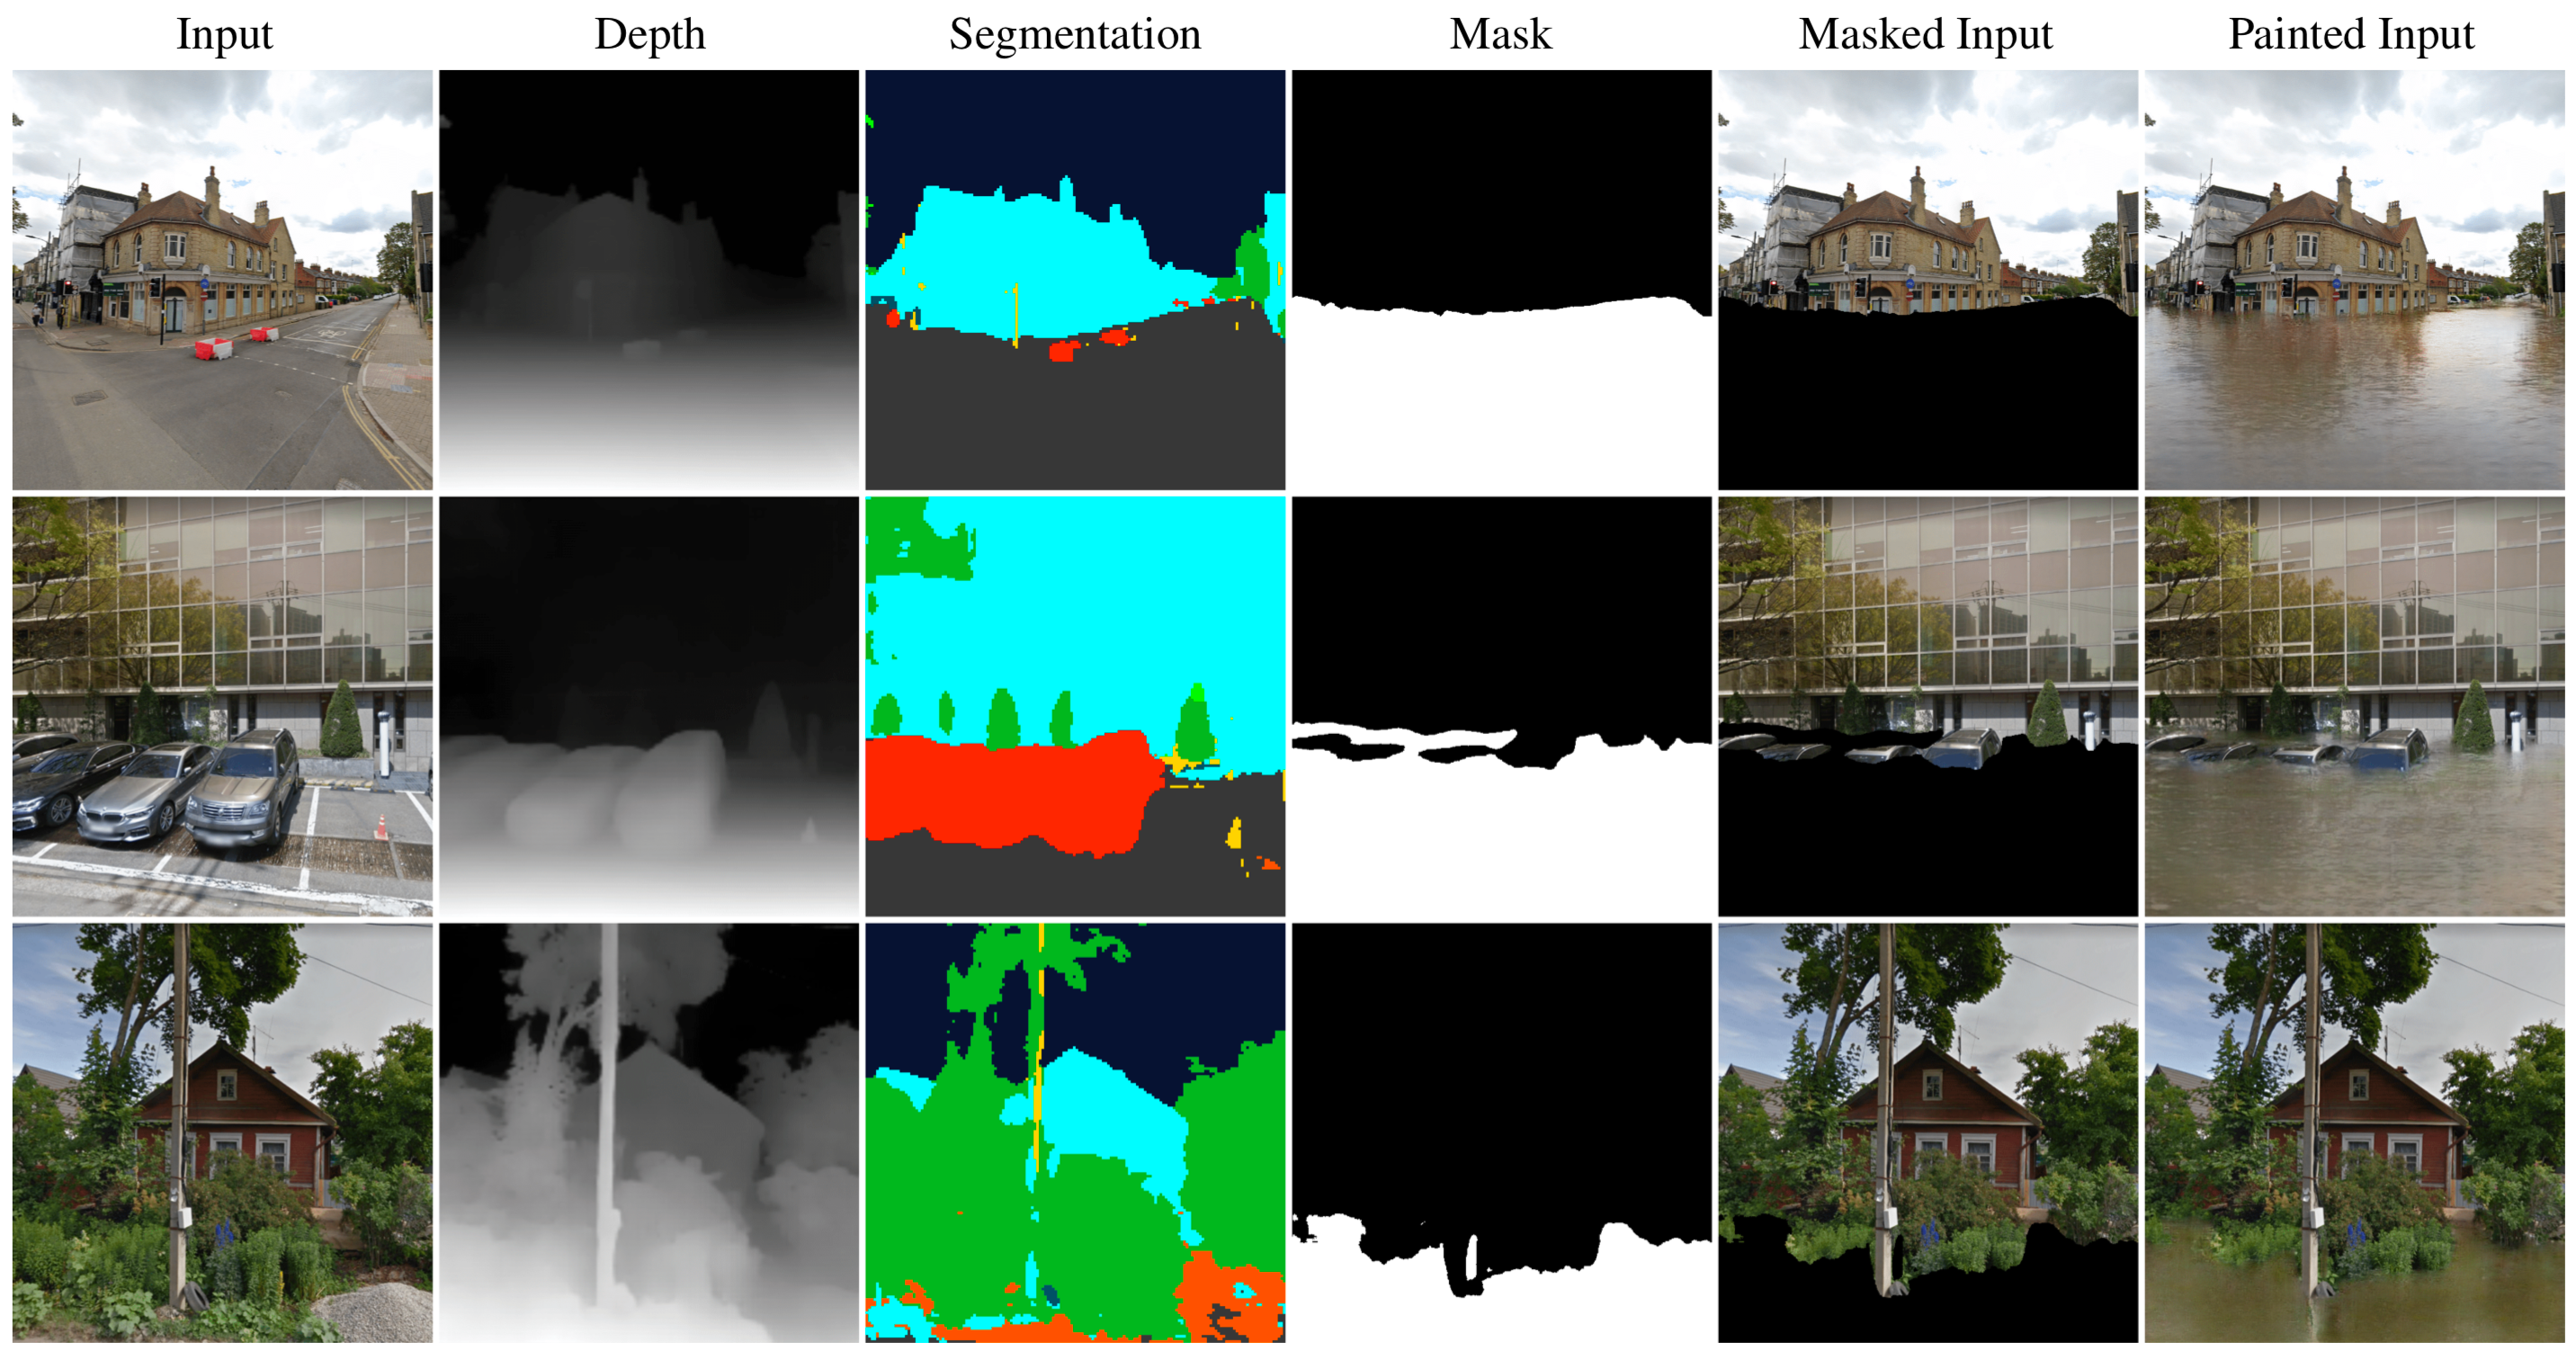
\includegraphics[scale=0.32]{images/ClimateGAN/flood.png}
        \caption[ClimateGAN pipeline]{Pipeline for creating photorelistic images with flood proposed by \citet[p.6]{climategan}. Reusing the segmentation map for generating the mask of the road and the depth map for calculating the flatness of the ground}
        \label{fig:flood_representation}
    \end{figure}
    
    To create a dataset for bench-marking we used images from the validation dataset of \acrshort{bdd} to create a dataset of images with the flood, wild-fire, and dense-smog. Combining the \acrshort{idd} and the ClimateGAN model generated images we generated a dataset and from further on the dataset is referred to as $OD^{2}$ (Out-of-Distribution detection for Object Detection). 
    
    % \begin{figure}[H]
    %     \captionsetup[subfigure]{labelformat=empty}
    %     \begin{tabular}{cccc}
    %         \subfloat{\includegraphics[width = 1.4in]{images/ClimateGAN/bdd/ba9f23d8-a50cd80e_normal_1024.png}} &
    %         \subfloat{\includegraphics[width = 1.4in]{images/ClimateGAN/bdd/ba9f23d8-a50cd80e_flood_1024.png}} &
    %         \subfloat{\includegraphics[width = 1.4in]{images/ClimateGAN/bdd/ba9f23d8-a50cd80e_wildfire_1024.png}} &
    %         \subfloat{\includegraphics[width = 1.4in]{images/ClimateGAN/bdd/ba9f23d8-a50cd80e_smog_1024.png}}
    %     \end{tabular}
    % \end{figure}
    
    \begin{figure}
        \captionsetup[subfigure]{labelformat=empty}
        \begin{tabular}{cccc}
            \subfloat{\includegraphics[width = 1.4in]{images/ClimateGAN/bdd/b1c9c847-3bda4659_normal_1024.png}} &
            \subfloat{\includegraphics[width = 1.4in]{images/ClimateGAN/bdd/b1c9c847-3bda4659_flood_1024.png}} &
            \subfloat{\includegraphics[width = 1.4in]{images/ClimateGAN/bdd/b1c9c847-3bda4659_wildfire_1024.png}} &
            \subfloat{\includegraphics[width = 1.4in]{images/ClimateGAN/bdd/b1c9c847-3bda4659_smog_1024.png}}\\
            \subfloat{\includegraphics[width = 1.4in]{images/ClimateGAN/bdd/b1c81faa-3df17267_normal_1024.png}} &
            \subfloat{\includegraphics[width = 1.4in]{images/ClimateGAN/bdd/b1c81faa-3df17267_flood_1024.png}} &
            \subfloat{\includegraphics[width = 1.4in]{images/ClimateGAN/bdd/b1c81faa-3df17267_wildfire_1024.png}} &
            \subfloat{\includegraphics[width = 1.4in]{images/ClimateGAN/bdd/b1c81faa-3df17267_smog_1024.png}}\\
            \subfloat{\includegraphics[width = 1.4in]{images/ClimateGAN/bdd/b1c66a42-6f7d68ca_normal_1024.png}} &
            \subfloat{\includegraphics[width = 1.4in]{images/ClimateGAN/bdd/b1c66a42-6f7d68ca_flood_1024.png}} &
            \subfloat{\includegraphics[width = 1.4in]{images/ClimateGAN/bdd/b1c66a42-6f7d68ca_wildfire_1024.png}} &
            \subfloat{\includegraphics[width = 1.4in]{images/ClimateGAN/bdd/b1c66a42-6f7d68ca_smog_1024.png}}\\
            \subfloat{\includegraphics[width = 1.4in]{images/ClimateGAN/bdd/ba9f6c98-c7216bf4_normal_1024.png}} &
            \subfloat{\includegraphics[width = 1.4in]{images/ClimateGAN/bdd/ba9f6c98-c7216bf4_flood_1024.png}} &
            \subfloat{\includegraphics[width = 1.4in]{images/ClimateGAN/bdd/ba9f6c98-c7216bf4_wildfire_1024.png}} &
            \subfloat{\includegraphics[width = 1.4in]{images/ClimateGAN/bdd/ba9f6c98-c7216bf4_smog_1024.png}}\\
            \subfloat[Normal]{\includegraphics[width = 1.4in]{images/ClimateGAN/bdd/baa03c1f-82d03594_normal_1024.png}} &
            \subfloat[Flood]{\includegraphics[width = 1.4in]{images/ClimateGAN/bdd/baa03c1f-82d03594_flood_1024.png}} &
            \subfloat[Wildfire]{\includegraphics[width = 1.4in]{images/ClimateGAN/bdd/baa03c1f-82d03594_wildfire_1024.png}} &
            \subfloat[Smog]{\includegraphics[width = 1.4in]{images/ClimateGAN/bdd/baa03c1f-82d03594_smog_1024.png}}
        \end{tabular}
        \caption[Sample image generated using ClimateGAN]{Samples from the dataset generated using ClimateGAN model and the images from the validation split of the \acrshort{bdd} dataset}
    \end{figure}
    
    \newpage
    \subsection{Performance Metrics}
    \label{benchmarking_metrics}
    In this section, we present various possible evaluation metrics that help in measuring the prediction quality when faced with OOD samples.
    
    \subsubsection{Area Under Receiver Operating characteristic Curve}
    \acrshort{auroc} is a measurement used to evaluate the performance of the classification problem at different thresholds. \acrshort{roc} is a probability curve, that is plotted between \acrlong{tpr} (\acrshort{tpr}) against \acrlong{fpr} (\acrshort{fpr}) and \acrshort{auroc} represents the measure of the classifiers ability to distinguish between the classes and can be used to summarize the \acrshort{roc} curve. The higher the \acrshort{auroc} value is the better is the classifier at the task under consideration. 
    
    This can be is used to evaluate the \acrshort{ood} detector that is posed as a classification problem as per the Equation \ref{id_vs_ood}. To pose the \acrshort{ood} detection as a classification problem,
    \begin{itemize}
        \item Assign a label of \textbf{0} to \acrlong{id} (\acrshort{id}) sample. 
        \item Assign a label of \textbf{1} to \acrshort{ood} sample.
        \item Use the novelty score that is provided by the \acrshort{ood} detector to perform the classification between \acrshort{id} and \acrshort{ood} samples.
    \end{itemize}
    
    The \acrshort{tpr} and \acrshort{fpr} values from the classification problem can be used to calculate the \acrshort{auroc} value that can represent the ability of the \acrshort{ood} detector in classifying \acrshort{OOD} and \acrshort{id} samples.
    
    \subsubsection{Probability and Entropy}
    \label{prob_entropy_calc}
    Entropy quantifies the uncertainty in the classification head of the network. Entropy is calculated using the Equation \ref{Entropy} from the mean of the softmax scores $s_{\mathbf{x}^{*}}$ as in Equation \ref{prob_calc} from each detection. 
    
    For an input $x^*$, the entropy and probability of a detection belonging to class $c$ among a total count of $C$ classes  is calculated using Equations \ref{prob_calc} and \ref{Entropy}. 
    
    \begin{equation}
            \label{prob_calc}
            \begin{aligned}
                p\left(c \mid \mathbf{x}^{*}\right) &= \frac{1}{N} \sum_{i=1}^{N} s_{\mathbf{x}^{*}}^{i}
            \end{aligned}
        \end{equation}
    
    \begin{equation}
        \label{Entropy}
        \begin{array}{l}
            \text{Entropy} =-\sum_{i=1}^{C} P\left(c_i \mid \mathbf{x}^{*} ; \mathcal{D}\right) \ln P\left(c_i \mid \mathbf{x}^{*} ; \mathcal{D}\right) 
        \end{array}
    \end{equation}
    
    \subsubsection{Box Deviation}
    \label{bdev_calc}
    Box deviation quantifies the uncertainty in bounding box regression. It represents how much each box $\hat{\mathbf{v}}_{\mathbf{x}^{*}}^{i}$ varies from their mean value. 
    
    \begin{enumerate}
        \item Final bounding box detections are calculated as the mean value of the detections regressed during N forward passes.
        \item Covariance matrix of the detections is calculated using the following the equation
            \begin{equation}
                C\left(\mathbf{x}^{*}\right)=\frac{1}{N} \sum_{i=1}^{N} \hat{\mathbf{v}}_{\mathbf{x}^{*}}^{i} \hat{\mathbf{v}}_{\mathbf{x}^{*}}^{i^{T}}-\mathbf{I}_{\mathbf{x}^{*}} \mathbf{I}_{\mathbf{x}^{*}}^{T}
            \end{equation}
        \item Box deviation is the square root of the trace of the covariance matrix $C(x^{*})$.
    \end{enumerate}
         
    The box deviations span from $[0,+\infty)$, the higher the value represents the higher the epistemic uncertainty in regressed bounding box parameters.
    
    \section{Out-of-Distribution for Object Detection ($OD^{2}$) Dataset Summary}
    In this section, we summarize the key features of the proposed $OD^{2}$ dataset along with the method used to compare various \acrshort{ood} methods for object detection.
    
    To test the performance of \acrshort{ood} detector on images:
    \begin{enumerate}
        \item In case of a low-quality image, we propose the usage of images with various weather conditions like partly cloudy, foggy, overcast, etc. To confirm that all types of objects are present in the images, we also propose the usage of smog-filled images generated using Climate-GAN. 
        \item From a different domain, we propose the usage of images with fire and flood overlay produced using Climate-GAN along with images from \acrshort{idd} dataset.
        \item with novel classes, we propose the usage of images from \acrshort{idd} dataset with Auto-Rickshaws.
    \end{enumerate}
    
    \subsubsection{Task Description}
    This section outlines the tasks we are planning to achieve using $OD^2$ dataset
    \begin{description}
        \item[Object Detector Performance] This task ensures the object detector's performance on the closed dataset that is chosen for training purposes. In $OD^2$ dataset this is achieved using the test split of the \acrshort{bdd} dataset.
        \item[Detector Robustness] This task is similar to task 1. Except, the data that is used for inference is from a different but plausible weather condition.
        \item[\acrshort{ood} Detection] This task is to detect the samples which are from a known data distribution but are semantically different from the data used for training.
        \item[Multi-class Novelty Detection] This task is to quantify the ability of \acrshort{ood} detector to produce high novelty scores for unknown-unknown samples. The class of Auto-Rickshaw in \acrshort{idd} dataset helps in evaluating this task.
        \item[Out-of-Domain Detection] This task is to test the ability of the \acrshort{ood} detection methods to provide high novelty scores when the input sample is from a different domain to the training dataset. The Flood and WildFire datasets generated can be used to serve this purpose.
    \end{description}
    
    The $OD^{2}$ dataset can be summarised as shown in Table \ref{dataset_summary}
    
    \begin{table}[H]
        \centering
        \renewcommand{\arraystretch}{1.25}
        \caption{Table showing various type of images to address the \acrshort{ood} cases presented in Section \ref{ood_cases}. The table also show the sources of the images that are collected from along with the expected behavior of the novelty score for each \acrshort{ood} class of dataset}
        \begin{adjustbox}{width=1\textwidth}
            \begin{tabular}{lllll}
            \hline
            \textbf{Purpose} & \textbf{Dataset Source} & \textbf{Classes} & \textbf{Novelty Score Behavior} & Task \\ \hline
            In-Distribution & BDD100K & \begin{tabular}[c]{@{}l@{}}Pedestrian, Rider, Car, Truck, Bus, \\ Motorcycle, Bicycle, Traffic sign\end{tabular} & Low Novelty score  & \begin{tabular}[c]{@{}l@{}}Object detector \\ performance \end{tabular} \\ \hline
            \begin{tabular}[c]{@{}l@{}}Low light and \\ bad image quality\end{tabular} & \begin{tabular}[c]{@{}l@{}}BDD100K (non-clear weather) \\ and Climate-GAN generated \\ Smog images\end{tabular} & \begin{tabular}[c]{@{}l@{}}Pedestrian, Rider, Car, Truck, Bus, \\ Motorcycle, Bicycle, Traffic sign\end{tabular} & Medium Novelty Score   & Detector Robustness\\ \hline
            \begin{tabular}[c]{@{}l@{}}Classes with \\ semantic-variance\end{tabular}  & IDD & Trucks, Motorcycles, Traffic Sign & High Novelty Score     & \acrshort{ood} detection\\ \hline
            Novel Classes  & IDD & Auto-Rickshaws  & High Novelty Score     & \begin{tabular}[c]{@{}l@{}}Multi class \\ novelty detection \end{tabular} \\ \hline
            \begin{tabular}[c]{@{}l@{}}Out-of-Domain \\ images\end{tabular} & \begin{tabular}[c]{@{}l@{}}Climate-GAN generated \\ Flood and Fire images\end{tabular} & \begin{tabular}[c]{@{}l@{}}Pedestrian, Rider, Car, Truck, Bus, \\ Motorcycle, Bicycle, Traffic sign\end{tabular} & High Novelty Score & \begin{tabular}[c]{@{}l@{}}Out-Of-Domain \\ detection \end{tabular}\\ \hline
            \end{tabular}
        \end{adjustbox}
        \label{dataset_summary}
    \end{table}
    
\end{document}
